\startfirstchapter{Introduction}
\label{chapter:introduction}

The Standard Model (SM) of particle physics is the most complete theory that exists to describe elementary particles and their interactions. However there are known weaknesses in the SM, one of which is the failure to include a description of dark matter (DM). There is strong evidence from astronomical observations that there is a large excess of matter in the universe that appears to have only gravitational interactions with SM particles. Some examples for the evidence of dark matter include measurements of rotation velocities of spiral galaxies, gravitational lensing effects, and anisotropies in the cosmic microwave background. The standard model of cosmology predicts that dark matter accounts for approximately 27\% of the total mass energy of the universe. Although there are many theories to describe possible dark matter candidates, the one of interest here is the WIMP (weakly interacting massive particle). The WIMP, often denoted $\chi$, is predicted to interact gravitationally and through other force(s), potentially beyond the SM, with a mass between 10 GeV and upwards of a few TeV. It is also predicted to have a self-annihilation cross section similar to that of SM weak interactions.

There are three types of experimental setups with the potential to observe dark matter. The first is direct detection experiments. These types of detectors look for recoils in SM particles from interacting with a DM particle.

\begin{figure}[htbp]
\centering
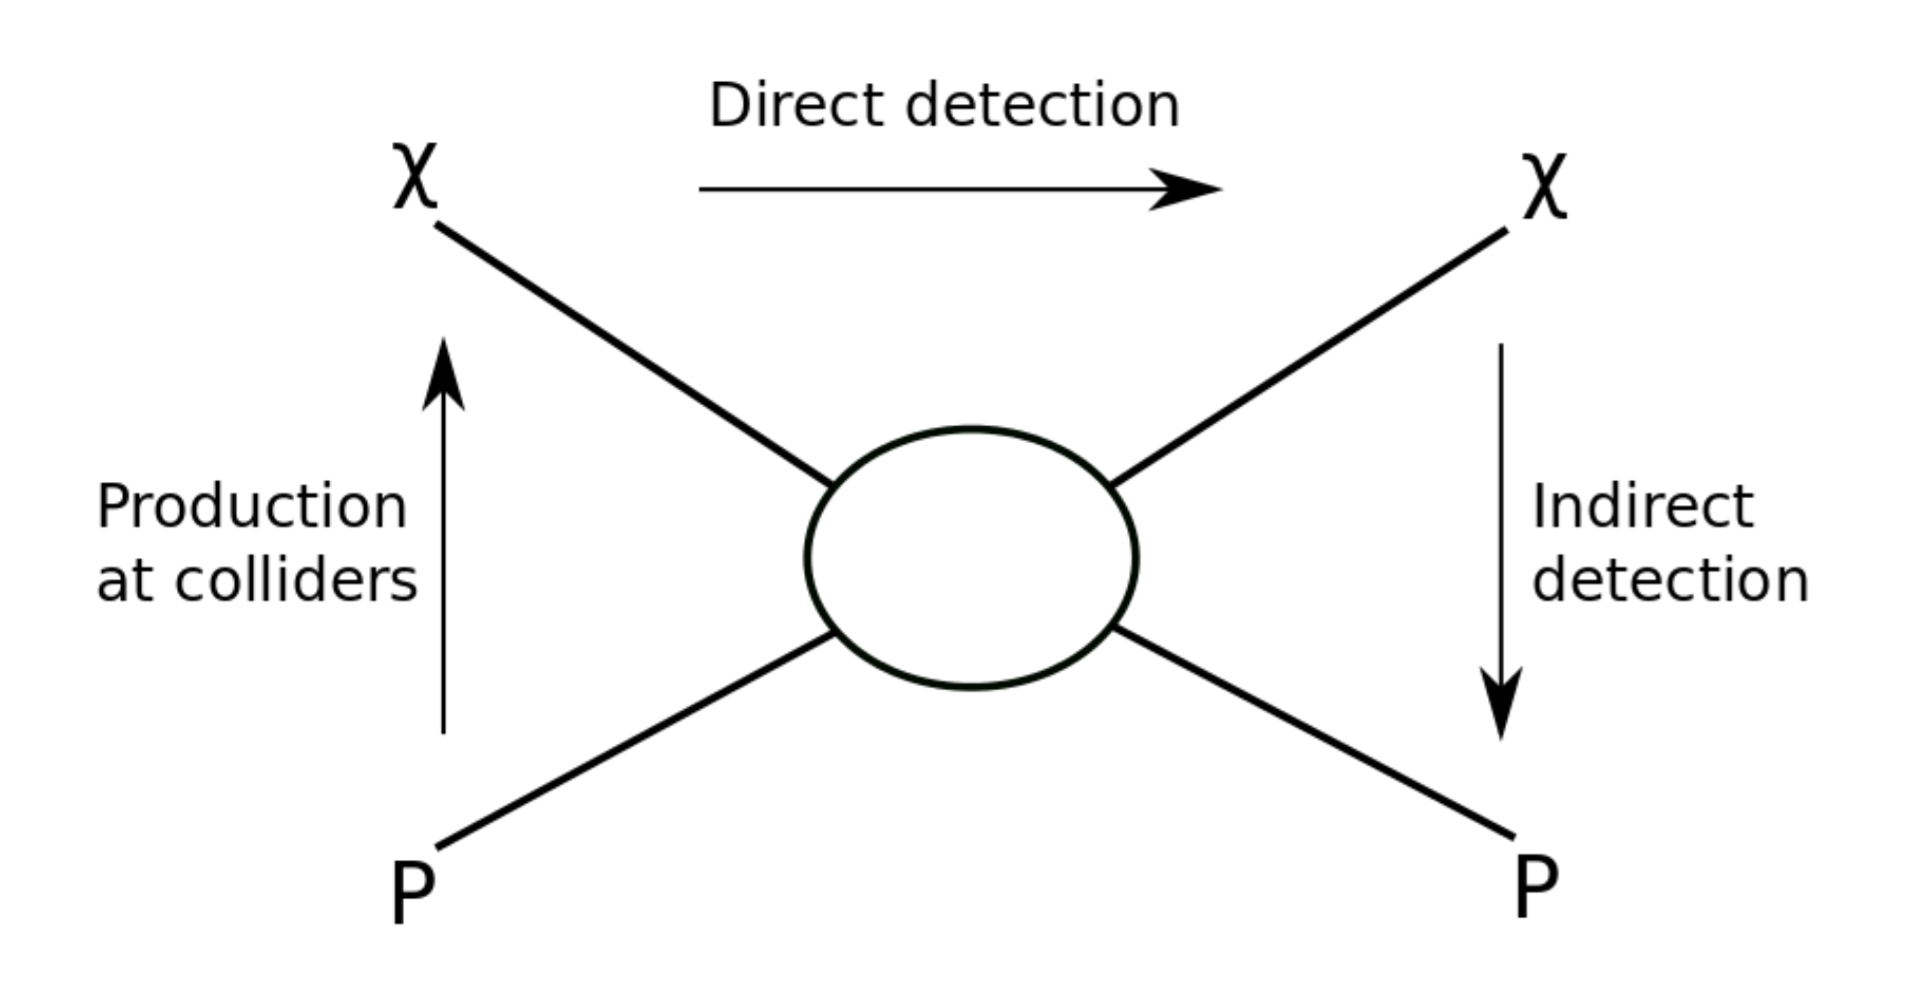
\includegraphics[width=0.7\textwidth]{Figures/DMDetection.png}
% https://arxiv.org/pdf/1509.08767.pdf
\caption{hi}
\label{fig:DMDetection}
\end{figure}



- dark matter production in colliders, complementarity to DD and ID\\
- missing transverse momentum, use of Z as a tag\\
- a signal would manifest as an excess of events with significant MET\\
- major backgrounds, systematics, limits\\
- mention results so far for ICHEP 2016 and EPS 2017, and for DM summary paper\\
- mention full Run 2 dataset prospects\\
- outline of document\\